\documentclass[handout]{beamer}
%\usepackage{pgfpages}
%\pgfpagesuselayout{4 on 1}[a4paper, landscape, border shrink=5mm]
%\pgfpageslogicalpageoptions{1}{border code=\pgfusepath{stroke}}
%pgfpageslogicalpageoptions{2}{border code=\pgfusepath{stroke}}
%\pgfpageslogicalpageoptions{3}{border code=\pgfusepath{stroke}}
%\pgfpageslogicalpageoptions{4}{border code=\pgfusepath{stroke}}
%\documentclass{beamer}
%\usetheme{nesl}  % Now it's a beamer presentation with the NESL theme!
\usetheme{Warsaw}
\usepackage{tikz}
\usetikzlibrary{shapes,arrows}
\usepackage{url}
\usepackage{verbatim}
\usefonttheme{serif}

% Make a new command that will make a new subsection and a frame with the same title
\newcommand{\fst}[2]{\subsection{#1}\frame{\frametitle{#1} #2}}

% Standard LaTeX stuff - note the optional abbreviated title being provided
\title{WRF Data Assimilation System}
\author[Zhang and Huang]{Xin Zhang \and Xiang-Yu Huang}

\date{April 16, 2011\\
5th East Asia WRF Tutorial
  ~\\
  ~\\
  ~\\
  ~\\
 \small{NCAR is sponsored by the National Science Foundation}
}

\institute[NCAR Earth System Laboratory]{
%  \url{mailto:xinzhang@ucar.edu} \\
   NCAR Earth System Laboratory \\
  ~\\
%  \url{ook@ucw.cz}\\
%  Charles University, Prague
}

% We want the NSF department logo
\logo{\includegraphics[height=.3in]{NSF_NESL.jpg}}

% Define block styles
\tikzstyle{minim} = [rectangle, draw, fill=gray!20, rounded corners,
    text width=8em, text centered, node distance=4.4cm, minimum height=2em]
\tikzstyle{runningminim} = [rectangle, draw, fill=green!100, rounded corners,
    text width=8em, text centered, node distance=4.4cm, minimum height=2em]
\tikzstyle{ana} = [rectangle, draw, fill=blue!20, node distance=4.0cm, 
    text width=3.7em, text centered, rounded corners, minimum height=2em]
\tikzstyle{runningana} = [rectangle, draw, fill=green!100, node distance=4.0cm, 
    text width=3.7em, text centered, rounded corners, minimum height=2em]
\tikzstyle{block} = [rectangle, draw, fill=blue!20, node distance=2.1cm, 
    text width=3.7em, text centered, rounded corners, minimum height=2em]
\tikzstyle{runningblock} = [rectangle, draw, fill=green!100, node distance=2.1cm, 
    text width=3.7em, text centered, rounded corners, minimum height=2em]
\tikzstyle{line} = [draw, very thick, color=black!50, -latex']
\tikzstyle{cloud} = [draw, ellipse,fill=red!20, node distance=1.5cm,
    minimum height=1.5em, text width=2.5em, text centered]

\newcommand{\wrfdaFlow}{
    % Place node
    \node [block] (setupFrame) (setupFrame){Setup\\Frame};
    \node [block, right of=setupFrame] (readNml) {Read\\namelist};
    \node [cloud, above of=readNml] (nml) {namelist};
    \node [block, right of=readNml] (setupBg) {Setup\\Background};
    \node [cloud, above of=setupBg] (xb) {$\mathbf{x}_b$};
    \node [block, right of=setupBg] (setupBE) {Setup\\Background\\Error};
    \node [cloud, above of=setupBE] (b0) {$\mathbf{B}$};
    \node [block, right of=setupBE] (setupOb){Setup\\Observations\\ \& Errors};
    \node [cloud, above of=setupOb] (yo) {$\mathbf{y}$};
    \node [block, below of=setupOb] (calInnov){Calculate\\$\mathbf{y}-H(\mathbf{x}$)};
    \node [minim, left of=calInnov] (minim){Minimize Cost Function};
    \node [ana, left of=minim] (ana){Compute\\Analysis};
    \node [block, below of=ana] (calDia){Calculate\\Diagnostics};
    \node [cloud, below of=calDia] (diagFiles) {Diag. Files};
    \node [block, right of=calDia] (output){Output\\Analysis};
    \node [cloud, below of=output] (xa) {$\mathbf{x}^a$};
    \node [block, right of=output] (tidyUp){Tidy Up};
    % Draw edges
    \path [line] (setupFrame) -- (readNml);
    \path [line] (nml) -- (setupFrame);
    \path [line] (nml) -- (readNml);
    \path [line] (readNml) -- (setupBg);
    \path [line] (xb) -- (setupBg);
    \path [line] (setupBg) -- (setupBE);
    \path [line] (b0) -- (setupBE);
    \path [line] (setupBE) -- (setupOb);
    \path [line] (yo) -- (setupOb);
    \path [line] (setupOb) -- (calInnov);
    \path [line] (calInnov) -- (minim);
    \path [line] (minim) -- (ana);
    \path [line] (ana) -- (calDia);
    \path [line] (calDia) -- (output);
    \path [line] (calDia) -- (diagFiles);
    \path [line] (output) -- (xa);
    \path [line] (output) -- (tidyUp);
}

\begin{document}

% The title page
\frame{\titlepage}

%%%%%%%%%%%%%%%%%%%%%%%%%
\section{WRFDA Basics}

\frame{
\frametitle{What is WRFDA ?}
\begin{itemize}
	\item WRFDA : A Data Assimilation system for WRF (ARW) model
	\begin{itemize}
		\item[-] Variational and Ensemble methods
		\item[-] Used for both research and operational data analysis
	\end{itemize}
	\item It is a supported �community model�, i.e. a 
free and shared resource with distributed 
development and centralized support
\end{itemize}
}

\frame{
\begin{center}
\includegraphics[scale=0.45]{wrfFlowChart}
\end{center}
}

\begin{comment}

\fst{WRFDA Applications}{
 \vspace{.1in}
\begin{tabular}{l p{2in}}
    {\mathbf Goal:} Community WRF DA system for \\
    \hspace{0.1in}  $\cdot$ regional/{\color{blue}global} \\
     \hspace{0.1in} $\cdot$ research/operations, and \\
     \hspace{0.1in} $\cdot$ deterministic/probabilistic applications\\
    {\mathbf Techniques:} \\
    \hspace{0.1in}  $\cdot$ 3D-Var \\
     \hspace{0.1in} $\cdot$ 4D-Var (regional) \\
     \hspace{0.1in} $\cdot$ {\color{blue} Ensemble DA} \\
     \hspace{0.1in} $\cdot$ {\color{blue} Hybrid Variational/Ensemble DA} 
     &  \vspace{-1.4in}  \includegraphics[height=1.0in, viewport=10 20 280 185, clip]{cwb_domain.png} \\
    {\mathbf Model:} WRF (ARW, {\color{blue} NMM, Global}) & \\
    {\mathbf Support:} \\
     \hspace{0.1in} $\cdot$ NCAR/ESL/MMM/DAS \\
     \hspace{0.1in} $\cdot$  NCAR/RAL/JNT/DATC & \vspace{-1.0in}  \includegraphics[height=1.05in]{AFWA_domain.png}   \\
    {\mathbf Observations:} Conv. + Sat. + Radar & \vspace{-.5in} 
\end{tabular}
}

\end{comment}

\fst{ WRFDA formulation}{
\begin{equation*}
J=\frac{1}{2}(\mathbf{x}-\mathbf{x}_b)^T{\mathbf{B}^{-1}}(\mathbf{x}-\mathbf{x}_b)+\frac{1}{2}[\mathbf{y}_o-\textsl{H}(\mathbf{x})]^T\mathbf{R}^{-1}[\mathbf{y}_o-\textsl{H}(\mathbf{x})]
\end{equation*} \pause
Define the first guess of the $n^{th}$ outer loop: $\mathbf{x}_{n-1}$, note: $\mathbf{x}_0=\mathbf{x}_b$\pause
\begin{align*}
J &=\frac{1}{2}(\mathbf{x}_n-\mathbf{x}_{n-1}+\mathbf{x}_{n-1}-\mathbf{x}_b)^T{\mathbf{B}^{-1}}(\mathbf{x}_n-\mathbf{x}_{n-1}+\mathbf{x}_{n-1}-\mathbf{x}_b) \\
   & +\frac{1}{2}[\mathbf{y}_o-\textsl{H}(\mathbf{x}_n)]^T\mathbf{R}^{-1}[\mathbf{y}_o-\textsl{H}(\mathbf{x}_n)]
\end{align*} \pause
Define analysis increment of $n^{th}$ outer loop: $\delta\mathbf{x}_n=\mathbf{x}_n-\mathbf{x}_{n-1}$ \pause
\begin{align*}
J &= \frac{1}{2}(\delta\mathbf{x}_n+\mathbf{x}_{n-1}-\mathbf{x}_b)^T{\mathbf{B}^{-1}}(\delta\mathbf{x}_n+\mathbf{x}_{n-1}-\mathbf{x}_b) \\
   &+\frac{1}{2}[\mathbf{y}_o-\textsl{H}(\mathbf{x}_{n-1}+\delta\mathbf{x}_n)]^T\mathbf{R}^{-1}[\mathbf{y}_o-\textsl{H}(\mathbf{x}_{n-1}+\delta\mathbf{x}_n)]
\end{align*}
}

\begin{frame}
Define innovation : $\mathbf{d}_{n}=\mathbf{y}_o-\textsl{H}_{n-1}(\mathbf{x}_{n-1})$ \pause
\begin{align*}
J &= \frac{1}{2}(\delta\mathbf{x}_n+\mathbf{x}_{n-1}-\mathbf{x}_b)^T{\mathbf{B}^{-1}}(\delta\mathbf{x}_n+\mathbf{x}_{n-1}-\mathbf{x}_b) \\
    &+\frac{1}{2}[\mathbf{d}_{n}-\mathbf{H}_{n-1}(\delta\mathbf{x}_n)]^T\mathbf{R}^{-1}[\mathbf{d}_{n}-\mathbf{H}_{n-1}(\delta\mathbf{x}_n)]
\end{align*}
$\mathbf{H}_{n-1}=\frac{\partial\textsl{H}_{n-1}}{\partial\mathbf{x}_{n-1}}$ is the tangent linear observational operator \\ \pause
To find the $\delta\mathbf{x}_n$ which lead $J$ to minimium:
\begin{equation*}
\nabla_{\delta\mathbf{x}_n}{J}=0
\end{equation*}
\begin{equation*}
\nabla_{\delta\mathbf{x}_n}{J}=\mathbf{B}^{-1}(\delta\mathbf{x}_n+\mathbf{x}_{n-1}-\mathbf{x}_b)-\mathbf{H}_{n-1}^T\mathbf{R}^{-1}(\mathbf{d}_n-\mathbf{H}_{n-1}(\delta\mathbf{x}_n))
\end{equation*}
\end{frame}

\begin{frame}
At the minimium, $\nabla_{\delta\mathbf{x}_n}{J}$ vanishes:
\begin{align*}
(\mathbf{B}^{-1}+\mathbf{H}_{n-1}^T\mathbf{R}^{-1}\mathbf{H}_{n-1})\delta\mathbf{x}_n=\mathbf{H}_{n-1}^T\mathbf{R}^{-1}\mathbf{d}_{n}-\mathbf{B}^{-1}(\mathbf{x}_{n-1}-\mathbf{x}_b)
\end{align*} \pause
Then
\begin{align*}
\delta\mathbf{x}_n=(\mathbf{B}^{-1}+\mathbf{H}_{n-1}^T\mathbf{R}^{-1}\mathbf{H}_{n-1})^{-1}[\mathbf{H}_{n-1}^T\mathbf{R}^{-1}\mathbf{d}_n-\mathbf{B}^{-1}(\mathbf{x}_{n-1}-\mathbf{x}_b)]
\end{align*}
With the Woodbury Matrix Identity formulation: \\
\begin{center}
$(\mathbf{A}+\mathbf{UCV})^{-1}=\mathbf{A}^{-1}-\mathbf{A}^{-1}\mathbf{U}(\mathbf{C}^{-1}+\mathbf{V}\mathbf{A}^{-1}\mathbf{U})^{-1}\mathbf{V}\mathbf{A}^{-1}$
\end{center}
\begin{align*}
(\mathbf{B}^{-1}+\mathbf{H}_{n-1}^T\mathbf{R}^{-1}\mathbf{H}_{n-1})^{-1} =\mathbf{B}-\mathbf{B}\mathbf{H}_{n-1}^T(\mathbf{R}+\mathbf{H}_{n-1}\mathbf{B}\mathbf{H}_{n-1}^T)^{-1}\mathbf{H}_{n-1}\mathbf{B} 
\end{align*}
\end{frame}

\begin{frame}
\begin{align*}
\delta\mathbf{x}_n = & [\mathbf{B}-\mathbf{B}\mathbf{H}_{n-1}^T(\mathbf{R}+\mathbf{H}_{n-1}\mathbf{B}\mathbf{H}_{n-1}^T)^{-1}\mathbf{H}_{n-1}\mathbf{B}] \\
 & [\mathbf{H}_{n-1}^T\mathbf{R}^{-1}\mathbf{d}_n-\mathbf{B}^{-1}(\mathbf{x}_{n-1}-\mathbf{x}_b)]
\end{align*}
\begin{align*}
\delta\mathbf{x}_n= & \mathbf{B}\mathbf{H}_{n-1}^T(\mathbf{R}+\mathbf{H}_{n-1}\mathbf{B}\mathbf{H}_{n-1}^T)^{-1}[\mathbf{d}_n+\mathbf{H}_{n-1}(\mathbf{x}_{n-1}-\mathbf{x}_b)] \\
& - (\mathbf{x}_{n-1}-\mathbf{x}_b)
\end{align*}
Please note that the new analysis is : \\
\begin{center}
$\mathbf{x}_a=\delta\mathbf{x}+\mathbf{x}_{n-1}$
\end{center}
\end{frame}

\begin{frame}
For one outer loop, $\mathbf{x}_0=\mathbf{x}_b$ and $\mathbf{d}=\mathbf{y}_o-\textsl{H}(\mathbf{x}_b)$
\begin{equation*}
J = \frac{1}{2}\delta\mathbf{x}^T{\mathbf{B}^{-1}}\delta\mathbf{x}+\frac{1}{2}(\mathbf{d}-\mathbf{H}\delta\mathbf{x})^T\mathbf{R}^{-1}(\mathbf{d}-\mathbf{H}\delta\mathbf{x})
\end{equation*} \pause
\begin{equation*}
\nabla_{\delta\mathbf{x}}{J}=\mathbf{B}^{-1}\delta\mathbf{x}-\mathbf{H}^T\mathbf{R}^{-1}(\mathbf{d}-\mathbf{H}\delta\mathbf{x})
\end{equation*} \pause
\begin{equation*}
\delta\mathbf{x}=\mathbf{B}\mathbf{H}^T(\mathbf{R}+\mathbf{H}\mathbf{B}\mathbf{H}^T)^{-1}\mathbf{d}
\end{equation*}
\end{frame}

%%%%%%%%%%%%%%%%%%%%%%%%%
\section{WRFDA Overview}

\fst{Prepare the BE}{

\begin{equation*}
J = \frac{1}{2}\delta\mathbf{x}^T{\color{red}\mathbf{B}^{-1}}\delta\mathbf{x}+\frac{1}{2}(\mathbf{d}-\mathbf{H}\delta\mathbf{x})^T\mathbf{R}^{-1}(\mathbf{d}-\mathbf{H}\delta\mathbf{x})
\end{equation*} \pause
\begin{itemize}
\item Nominally, {\color{red}$\mathbf{B}$} is the background error covariance \pause
\item For initial testing, default background error statistics may
be used \pause 
\begin{itemize}
\item be.dat file (CV option 5) from test case tar file can \alert{only be used
with the case of online tutorial} \pause
\item be.dat.cv3 (CV option 3) from source code tar file can be used for
general test domains, \alert{tuning is still needed for satisfied performance}
\end{itemize} \pause
\item Ultimately, {\color{red}$\mathbf{B}$} should be specific to the particular
model domain (and season)
\end{itemize}

}

\fst{Prepare the Background}{

\begin{equation*}
J = \frac{1}{2}\delta\mathbf{x}^T{\color{blue}\mathbf{B}^{-1}}\delta\mathbf{x}+\frac{1}{2}(\mathbf{d}-\mathbf{H}\delta\mathbf{x})^T\mathbf{R}^{-1}(\mathbf{d}-\mathbf{H}\delta\mathbf{x})
\end{equation*} 
\begin{center}
$\delta\mathbf{x}=\mathbf{x}-{\color{red}\mathbf{x}_b}$
\end{center} \pause
\begin{itemize}
\item In �cold-start mode: accomplished by running the
WPS and real programs \pause
\begin{itemize}
\item The background is the wrfinput\_d01 file
\end{itemize} \pause
\item In �cycling mode: the output of the WRF model \pause
\begin{itemize}
\item WRF can output wrfinput-formatted files used for cycling 
\end{itemize}
\end{itemize}

}

\fst{Prepare the Observations \& Errors}{

\begin{equation*}
J = \frac{1}{2}\delta\mathbf{x}^T{\color{blue}\mathbf{B}^{-1}}\delta\mathbf{x}+\frac{1}{2}({\color{red}\mathbf{d}}-\mathbf{H}\delta\mathbf{x})^T{\color{red}\mathbf{R}^{-1}}(\mathbf{d}-\mathbf{H}\delta\mathbf{x})
\end{equation*}
\begin{center}
$\mathbf{d}={\color{red}\mathbf{y}}-\textsl{H}({\color{blue}\mathbf{x}_b})$
\end{center} \pause
\begin{itemize}
\item Conventional observation input for WRFDA is supplied through \pause
\begin{itemize}
\item Little\_R format, observation preprocessor, OBSPROC \pause
\item  Prepbufr format data directly \pause
\end{itemize} \pause
\item Observation error covariance also provided by OBSPROC (R is a diagonal matrix) \pause
\item \alert{Separate input file (ASCII) for radar, both reflectivity and radial velocity} \pause
\item \alert{Separate input file for satellite radiances, BUFR format} 
\end{itemize}

}

\fst{Run WRFDA}{

\begin{equation*}
J = \frac{1}{2}\delta\mathbf{x}^T{\color{blue}\mathbf{B}^{-1}}\delta\mathbf{x}+\frac{1}{2}({\color{blue}\mathbf{d}}-\mathbf{H}\delta\mathbf{x})^T{\color{blue}\mathbf{R}^{-1}}({\color{blue}\mathbf{d}}-\mathbf{H}\delta\mathbf{x})
\end{equation*}
\begin{itemize}
\item $H$ is the observational operator, which calculate the counterpart of observations in model space \pause
\item Conjuagate gradient method
\item Try to find a $\delta\mathbf{x}^a$ , which minimizes $J$ and then $\mathbf{x}^a=\mathbf{x}^b + \delta\mathbf{x}^a$
\end{itemize}

}

\fst{Update Boundary Condition}{

\begin{itemize}
\item After creating an analysis, $\mathbf{x}^a$, we have changed
the initial conditions for the model \pause
\item However, tendencies in wrfbdy\_d01 file are valid for background, $\mathbf{x}_b$ \pause
\item The update\_bc program adjusts these tendencies
based on the difference $\mathbf{x}^a - \mathbf{x}_b$ \pause
\item Of course, if $\mathbf{x}^a$ was produced for reasons other
than running WRF, there is probably not a need to
update boundary conditions
\end{itemize}

}

%%%%%%%%%%%%%%%%%%%%%%%%%%%%%%%%%

\section{WRFDA Implementation}

\begin{frame}
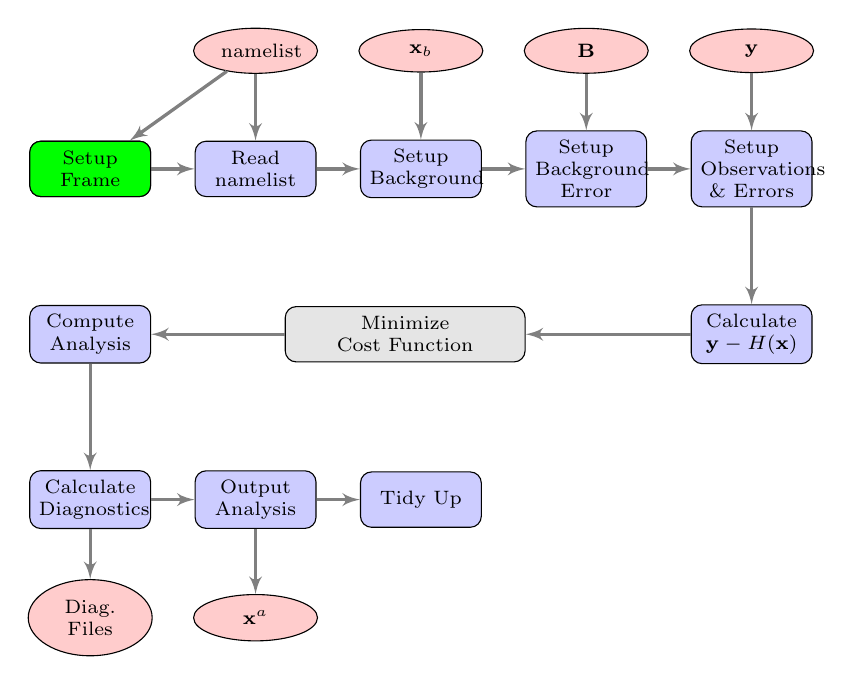
\begin{tikzpicture}[scale=1, node distance = 2.0cm, auto, font=\scriptsize]
\wrfdaFlow
\node [runningblock] (setupFrame) {Setup\\Frame};
\end{tikzpicture}
\end{frame}

\begin{frame}
\frametitle{Setup Frame}
\begin{itemize}
\item Reads grid dimensions from �$namelist.input$ file \pause
\item Use WRF framework� distributed memory capability to initialize tile, memory, patch dimensions, etc.
\end{itemize}
\end{frame}

\begin{frame}
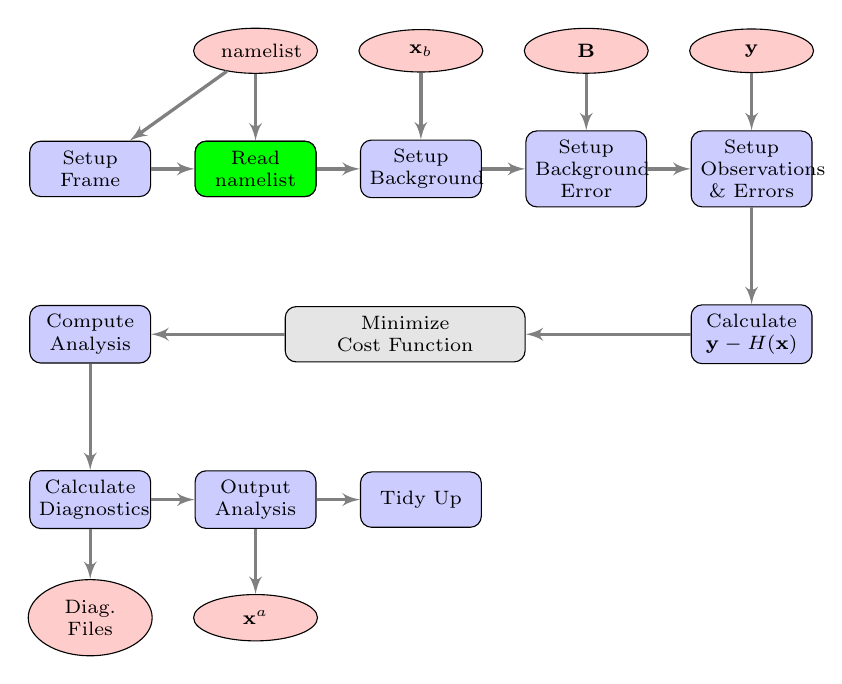
\begin{tikzpicture}[scale=1, node distance = 2.0cm, auto, font=\scriptsize]
\wrfdaFlow
\node [runningblock, right of=setupFrame] (readNml) {Read\\namelist};
\end{tikzpicture}
\end{frame}

\begin{frame}
\frametitle{Read namelist}
\begin{itemize}
\item Reads WRFDA data assimilation options from “namelist.input” file\pause
\item Performs consistency checks between namelist options.
\end{itemize}
\end{frame}

\begin{frame}
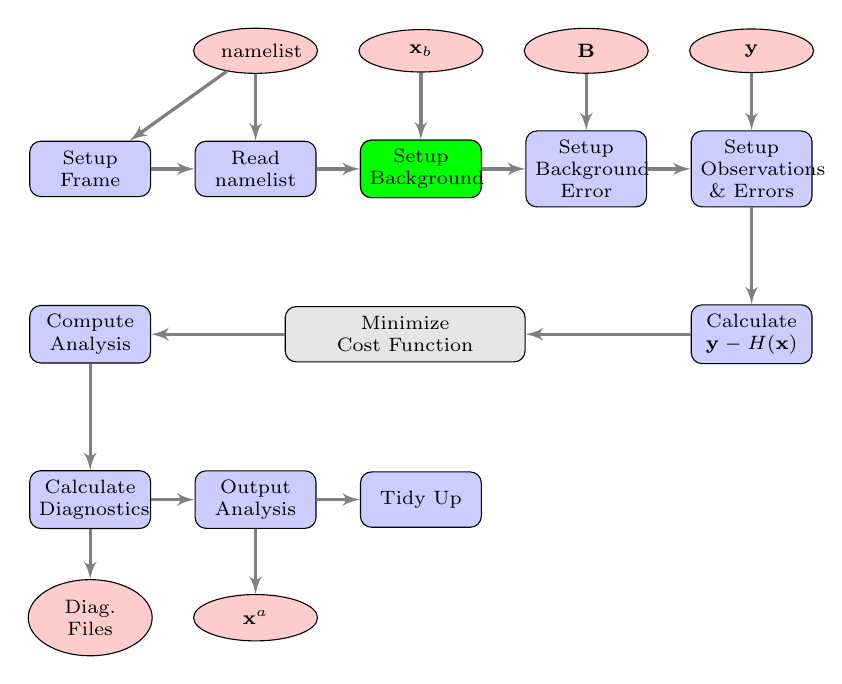
\begin{tikzpicture}[scale=1, node distance = 2.0cm, auto, font=\scriptsize]
\wrfdaFlow
\node [runningblock, right of=readNml] (setupBg) {Setup\\Background};
\end{tikzpicture}
\end{frame}

\begin{frame}
\frametitle{Setup Background}
\begin{itemize}
\item Reads the first-guess file \pause
\item Extracts fields used by WRFDA \pause
\item Creates background FORTRAN 90 derived data type $xb$ etc.
\end{itemize}
\end{frame}

\begin{frame}
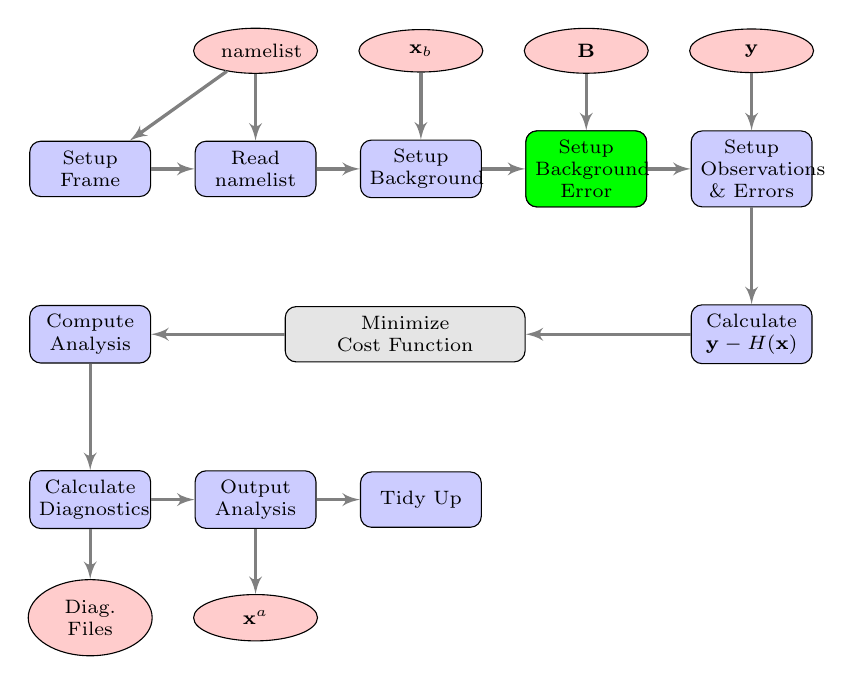
\begin{tikzpicture}[scale=1, node distance = 2.0cm, auto, font=\scriptsize]
\wrfdaFlow
\node [runningblock, right of=setupBg] (setupBE) {Setup\\Background\\Error};
\end{tikzpicture}
\end{frame}

\begin{frame}
\frametitle{Setup Background Error}
\begin{itemize}
\item Reads in background error statistics \pause
\item Extracts necessary quantities: eigenvectors, eigenvalues, lengthscales, regression coefficients, etc.\pause
\item Creates background error FORTRAN 90 derived data type $be$
\item Reference :\href{http://www.mmm.ucar.edu/wrf/users/wrfda/technotes.html}{{\bf{Online BE Documents}}}
\end{itemize}
\end{frame}

\begin{frame}
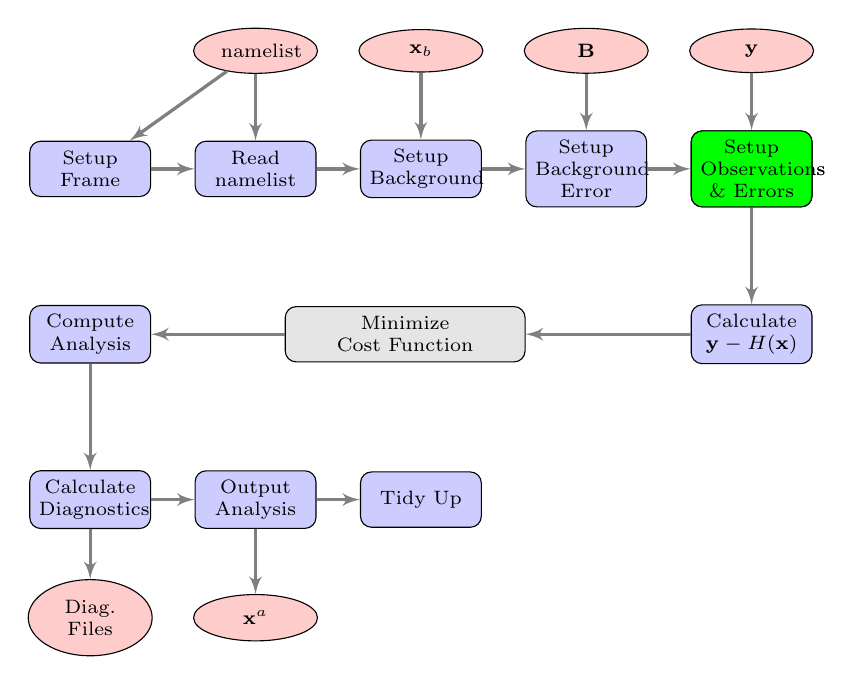
\begin{tikzpicture}[scale=1, node distance = 2.0cm, auto, font=\scriptsize]
\wrfdaFlow
\node [runningblock, right of=setupBE] (setupOb) {Setup\\Observations\\ \& Errors};
\end{tikzpicture}
\end{frame}

\begin{frame}
\frametitle{Setup Observations \& Errors}
\begin{itemize}
\item Reads in observations \pause
\item Assign observational error \pause
\item Creates observation FORTRAN 90 derived data type $ob$ \pause
\item Domain and time check
\end{itemize}
\end{frame}

\begin{frame}
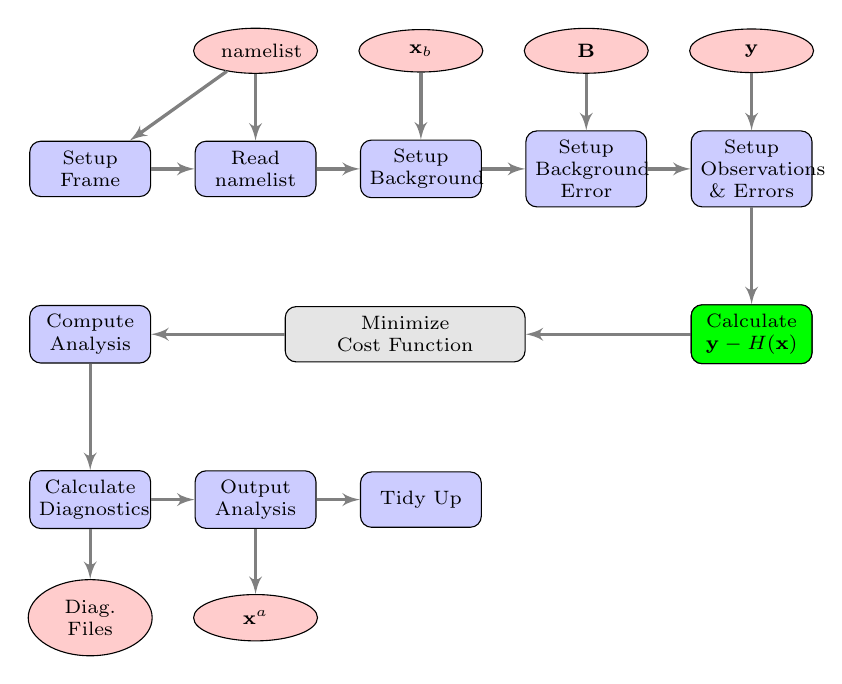
\begin{tikzpicture}[scale=1, node distance = 2.0cm, auto, font=\scriptsize]
\wrfdaFlow
\node [runningblock, below of=setupOb] (calInnov) {Calculate\\$\mathbf{y}-H(\mathbf{x})$};
\end{tikzpicture}
\end{frame}

\begin{frame}
\frametitle{Calculate Innovation}
\begin{itemize}
\item Calculates model equivalent of observations through interpolation and change of variable \pause
\item Computes observation minus first guess ($\mathbf{y}-H(\mathbf{x})$) value \pause
\item Creates innovation vector FORTRAN 90 derived data type $iv$
\end{itemize}
\end{frame}

\begin{frame}
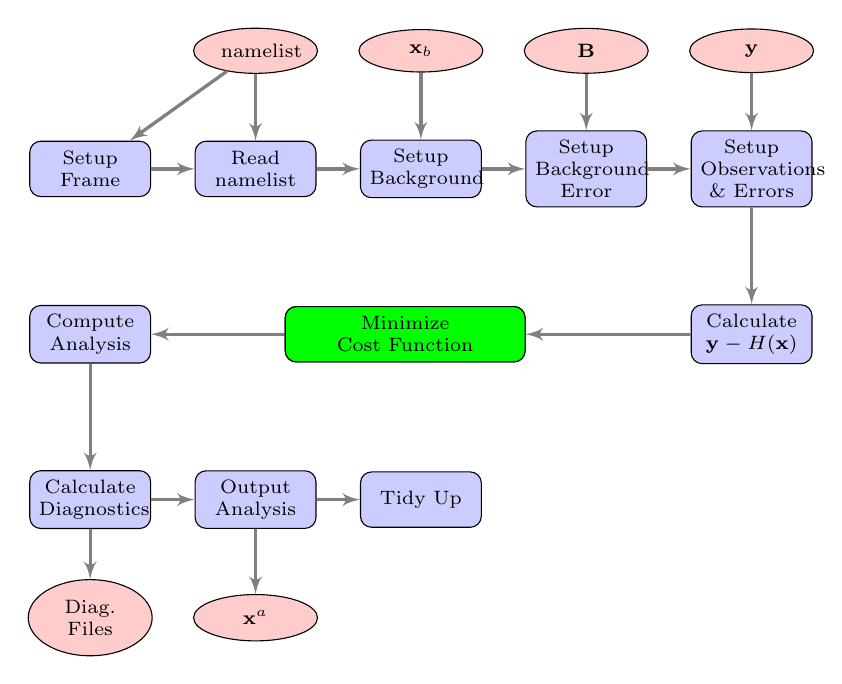
\begin{tikzpicture}[scale=1, node distance = 2.0cm, auto, font=\scriptsize]
\wrfdaFlow
\node [runningminim, left of=calInnov] (minim) {Minimize\\Cost Function};
\end{tikzpicture}
\end{frame}

\begin{frame}
\frametitle{Minimization}
Use conjugate gradient method \pause
\begin{itemize}
\item Initializes analysis increments to zero \pause
\item Computes cost function (if desired)\pause
\item Computes gradient of cost function \pause
\item Uses cost function and gradient to calculate new value of analysis control variable
\end{itemize}
\end{frame}

\begin{frame}
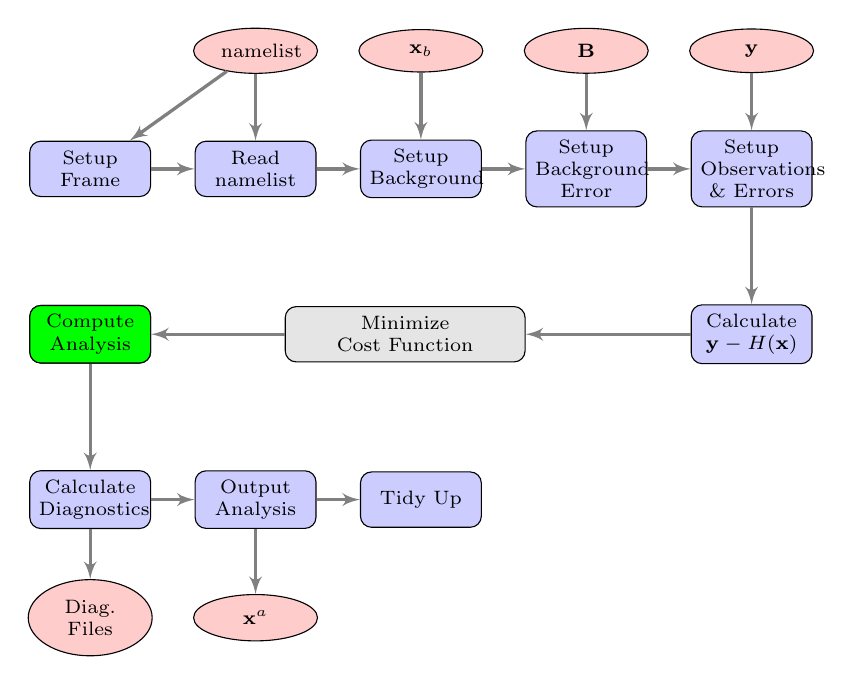
\begin{tikzpicture}[scale=1, node distance = 2.0cm, auto, font=\scriptsize]
\wrfdaFlow
\node [runningana, left of=minim] (ana) {Compute\\Analysis};
\end{tikzpicture}
\end{frame}

\begin{frame}
\frametitle{Compute Analysis}
\begin{itemize}
\item Once WRFDA has found a converged control variable, convert control variable to model space analysis increments \pause
\item Calculate:\\ 
            analysis = first-guess + analysis increment \pause
\item Performs consistency checks, e.g., remove negative humidity etc. \pause 
\item Optionally, do outer loop
\end{itemize}
\end{frame}

\begin{frame}
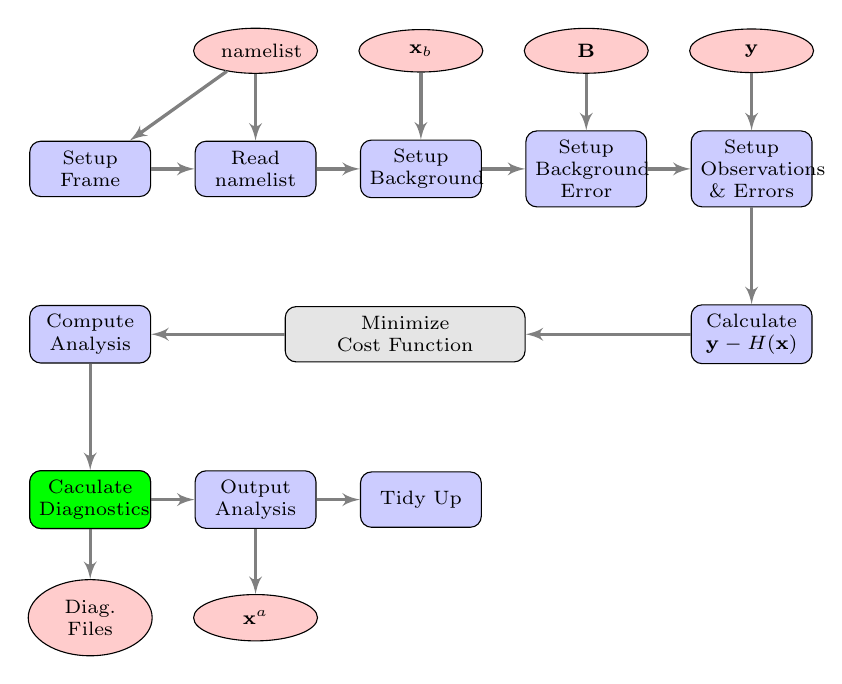
\begin{tikzpicture}[scale=1, node distance = 2.0cm, auto, font=\scriptsize]
\wrfdaFlow
\node [runningblock, below of=ana] (calDia) {Caculate\\Diagnostics};
\end{tikzpicture}
\end{frame}

\begin{frame}
\frametitle{Calculate Diagnostics}
\begin{itemize}
\item Output $\mathbf{y}-H(\mathbf{x}_b)$, $\mathbf{y}-H(\mathbf{x}^a)$ statistics for all observation types and variables \pause
\item Compute $\mathbf{x}^a-\mathbf{x}_b$ (analysis increment) statistics for all model variables and levels \pause
\item Statistics include minimum, maximum (and their locations), mean and standard deviation.
\end{itemize}
\end{frame}

\begin{frame}
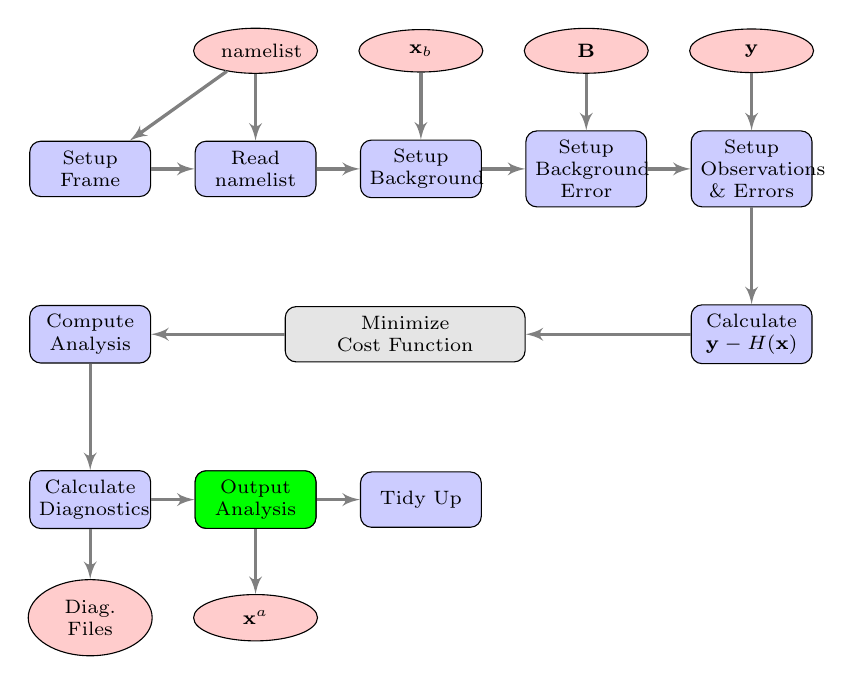
\begin{tikzpicture}[scale=1, node distance = 2.0cm, auto, font=\scriptsize]
\wrfdaFlow
\node [runningblock, right of=calDia] (output) {Output\\Analysis};
\end{tikzpicture}
\end{frame}

\begin{frame}
\frametitle{Output Analysis}
\begin{itemize}
\item Outputs analysis in native model format.
\end{itemize}
\end{frame}


\begin{frame}
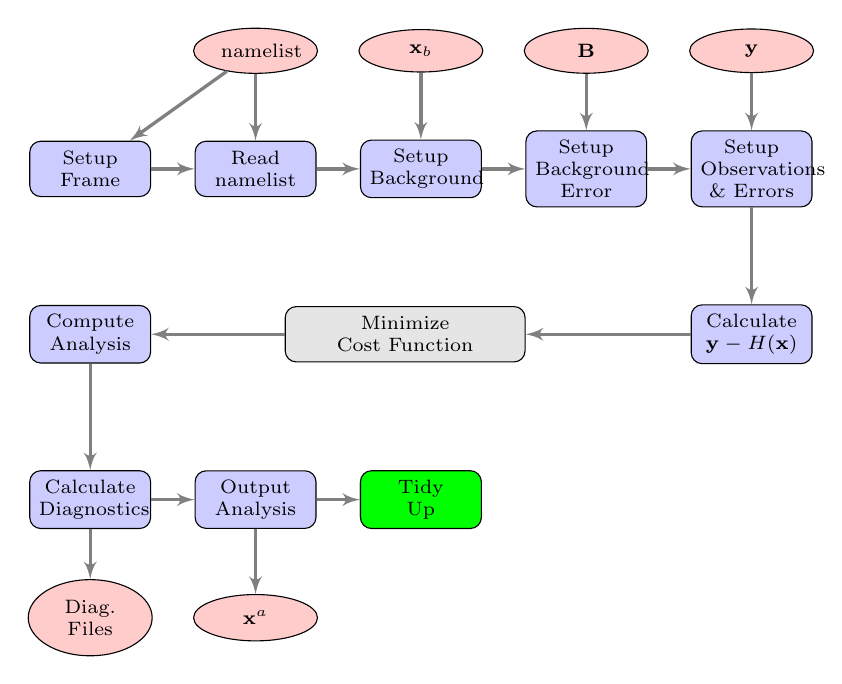
\begin{tikzpicture}[scale=1.0, node distance = 2.0cm, auto, font=\scriptsize]
\wrfdaFlow
\node [runningblock, right of=output] (tidyUp) {Tidy\\Up};
\end{tikzpicture}
\end{frame}

\begin{frame}
\frametitle{Tidy Up}
\begin{itemize}
\item Deallocate dynamically-allocated arrays, structures, etc.\pause
\item Timing information \pause
\item Clean end to WRFDA
\end{itemize}
\end{frame}

%%%%%%%%%%%%%%%%%%%%%%%%%%%%%%%%%
\section{WRFDA Software}

\fst{WRFDA Software Framework}{
\begin{center} 
\includegraphics[scale=0.4]{wrfSoftFrame}
\end{center}
\begin{itemize}
\item WRFDA relies on the WRF Software framework for \pause
\begin{itemize}
\item Distributed memory parallelism (halo exchanges, etc.)
\item Input/Output of first guess and analysis files 
\item Parallel transposes
\end{itemize} \pause
\item  WRFDA also uses \pause
\begin{itemize}
\item The WRF Registry mechanism to handle definitions of fields, halos, type, package and transposes {\color{red} (Registry.wrfvar)}
\item The WRF build system (clean, configure, compile)
\end{itemize}
\end{itemize}
}

\fst{WRFDA Code Organization}{
\begin{columns}[c]
\column{5cm}
\includegraphics[scale=0.4]{wrfdaCode}
\column{7cm}
\begin{block}{Remarks}
 \tiny{Besides the directories for WRF, the WRFDA tar file contains a $var$ directory, which holds all of the WRFDA code}
\end{block}
\end{columns}
}

\begin{frame}
\frametitle{WRFDA Code Organization}
\begin{columns}[c]
\column{5cm}
\includegraphics[scale=0.4]{wrfdaCode2}
\column{3cm}
\begin{block}{Remarks}
 \tiny{Generally, each subdirectory of $da$ contains a Fortran module with the same name}
\end{block}
\end{columns}
\end{frame}

\begin{frame}
\frametitle{WRFDA Code Organization}
\begin{columns}[c]
\column{5cm}
\includegraphics[scale=0.4]{wrfdaCode3}
\column{3cm}
\begin{block}{Remarks}
\begin{itemize}
\item  \tiny{da\_metar.f90 contains a Fortran module}
\item  \tiny{Each .inc file corresponds to a subroutine within the module}
\end{itemize}
\end{block}
\end{columns}
\end{frame}

\fst{Quick Start}{
\begin{itemize}
   \item Supported compilation mechanisms
   \begin{itemize}
    	\item Serial
     	\item Distributed-memory(dm)
     	\item Shared-memory(sm) {\color{red} (use with cautions, thread safe compiler only--IBM XLF )}
     	\item hybrid (dm+sm) {\color{red} (use with cautions )}
   \end{itemize}\pause
    \item Supported platforms
    \begin{itemize}
    	\item IBM: XLF
     	\item Linux: PGI, IFORT, {\color{red} GFORTRAN ( higher version needed,V4.4.0 tested )}
     	\item Macintosh intel: PGI, G95,  {\color{red} GFORTRAN ( higher version needed,V4.4.0 tested )}
    \end{itemize}\pause
    \item Included libraries
    \begin{itemize}
     	\item CRTM 2.0.2
	\item  BUFR, BLAS and LAPACK
    \end{itemize}
\end{itemize}
}

\begin{frame}
\begin{itemize}
	\item  Install NetCDF (V3.6 above) with {\color{red} THE SAME COMPILER} you will choose to compile WRFDA codes.\pause
	\item Setup the environmental variable
	\begin{itemize}
		\item csh, tcsh : setenv  NETCDF  $your\_netcdf\_path$
		\item bash, ksh : export  NETCDF=$your\_netcdf\_path$
	\end{itemize}\pause
	\item cd  WRFDA\pause
	\item ./clean -a\pause
	\item ./configure {\color{red}(-d)} wrfda {\color{red} (-d : compile with debug mode)}\pause
	\item ./compile all\_wrfvar\pause
	\item 41 executables should be generated under var/build directory
\end{itemize}
\end{frame}

\begin{frame}
\frametitle{ Upgraded to Mac OS X Snow Leopard Users }
\begin{itemize}
	\item PGI (v10.3.0, 64-bit), G95(v4.0.3, 32-bit), GFORTRAN(v4.4.0, default is 32-bit, '-m64' needed for 64-bit) have been tested. \pause
	\item gcc, g++ are verision 4.2.1, default is 64-bit, '-m32' needed for 32-bit. \pause
	\item NetCDF library should be re-install with appropriate compiler and option. \pause
        \item V3.3 configure is able to produce configure.wrf for PGI and G95. \pause
        \item For GFORTRAN compiler, '-m64' should be added to SFC,SCC, CCOMP in configure.wrf manually.\pause
        \item Prepbufr and Bufr format data have problem to be read on Snow Leopard system.
\end{itemize}
\end{frame}

\fst{Online WRFDA Resources}{
WRFDA has a dedicated page, similar to the ARW Users page: \href{http://www.mmm.ucar.edu/wrf/users/wrfda/}{{\bf WRFDA User Page}}
\begin{center}
\includegraphics[scale=0.4]{wrfdaHomePage}
\end{center}
}

\begin{frame}
\frametitle{Online Resources}
From the WRFDA page, one can access:
\begin{columns}[c, totalwidth=12cm]
\column{6cm}
\includegraphics[scale=0.4]{wrfdaDownload}
\column{6cm}
\includegraphics[scale=0.4]{wrfdaSystem}
\end{columns}
\begin{center}
\includegraphics[scale=0.4]{wrfdaDocPub}
\end{center}
\end{frame}

%%%%%%%%%%%%%%%%%%%%%%%%%%%%%%%%%%%
\fst{}{
\begin{center}
~\\
~\\
~\\
~\\
~\\
{\huge{\color{red}Thank You}}\\
~\\
~\\
~\\
~\\
~\\
{\tiny{\color{blue}The NESL Mission is: \\
To advance understanding of weather, climate, atmospheric composition and processes;\\
To provide facility support to the wider community; and, \\
To apply the results to benefit society.\\}}
~\\
{\small{NCAR is sponsored by the National Science Foundation}}
\end{center}
}

\end{document}
